\section{Visual Design Study}
\label{sec:visual_design}

\subsection{Type of visualization}
Gapminder is an Information Visualization (InfoVis) for the following reasons:
\begin{itemize}
    \item The domain of the data is discrete: Gapminder visualizes indicators measured over different countries in the world. The space of countries is clearly discrete.
    \item Data attributes have different types: some are categorical (e.g. countries), some are discrete (e.g. time in years), some are quantitative (e.g. average income). 
    \item The dimensionality of data values is high. We consider only $3$ indicators for each country, but the complete dataset of Gapminder has over $500$ indicators.
    \item All dimensions (except the geographical location) are time dependent, i.e. indicators are measured and vary over time.
    \item The visualization is interactive and has the scope to look for correlations between different indicators about the world situation.
\end{itemize}

Gapminder is clearly not a Scientific Visualization (SciVis).
SciVis data have a spatial domain, numerical values for the data attributes and a low dimension.

Gapminder is also clearly not a Infographic, since it is interactive and allows to explore different indicators.
Infographics are static, visualize summaries of the data and have the goal to present some content to a large audience.

\subsection{Visual encoding}
Gapminder offers $5$ different types of chart, called respectively: bubbles, maps, mountains, rankings and lines.
Since each chart uses visual variables in different ways, we analyze each of them separately.

For each chart, the screen is divided in different sectors:
a navigation bar in the top, the chart in the center, a slider at the bottom and a side bar on the right.

\begin{figure}[h]
	\centering
	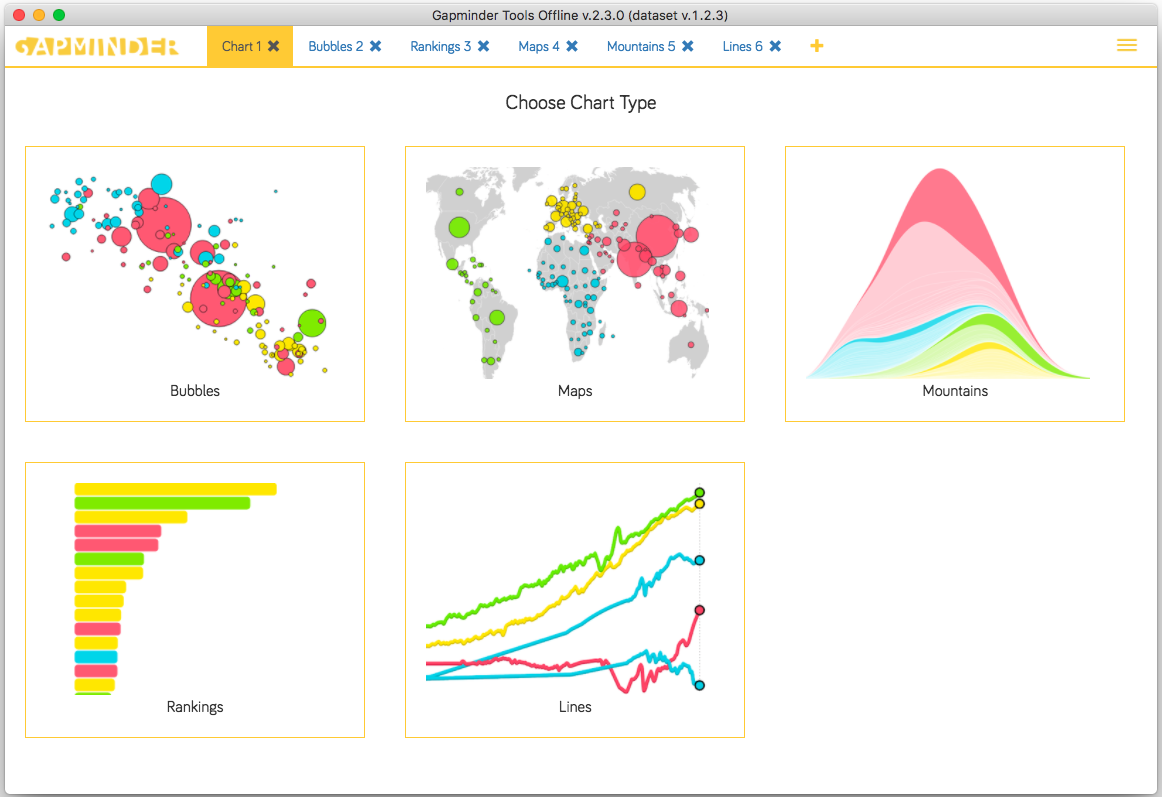
\includegraphics[width=0.95\columnwidth]{figures/home}
	\caption{Gapminder allows to work on multiple visualization at the same time. When creating a new chart, the user is asked to select the wanted type among the $5$ available.}
	\label{fig:home}
\end{figure}

\paragraph{Navigation}
Gapminder allows the user to create and use multiple charts at the same time: each chart is visualized as a tab in the navigation bar.
The navigation bar is located in the top part of the windows and is always visible.
The user can change the chart currently visualized by clicking the corresponding tab in the navigation bar.
To create a new chart, the user can use the \texttt{+} plus button at the end of the navigation bar.
When the user clicks the plus button, a new tab is created and displayed (\cref{fig:home}):
the user can choose a type of chart by clicking the correspondent button.

\paragraph{Right Panel}
The panel on the right contains different controls.
We will describe them from the top to the bottom.
At the very top, a menu allows the user to change the variable encoded as color.
Immediately below, Gapminder shows a colormap for the chosen variable.
Next we find a list of checkbox, one for each country.
This is a filter: it allows the user to select or deselect the countries to show.
At the very bottom there are some buttons that allows to control the zoom level, change the settings or activate the presentation mode.
Depending on the type of chart, Gapminder shows additional buttons in this area;
we will discuss this aspect in the sections about each chart's type.

\paragraph{Chart}
In the center-left part of the screen there is the current chart.
The chart occupies most of the area available on the screen.

\paragraph{Bottom Slider}
In the bottom part of the screen we find a ``play'' button and a time slider.
The button is used to start and stop the animation.
The slider allows to manually change the visualized year.


\subsubsection{Bubbles}
\label{subsubsec:bubbles}
Gapminder's ``bubbles'' are bubble charts with animations.
We consider the particular instance of bubble chart with the income on the x-axis, the life expectation on the y-axis and the population size encoded as the bubbles size; this is the default visualization offered by Gapminder when creating a new chart of type ``bubbles''.

\begin{figure}[h]
	\centering
	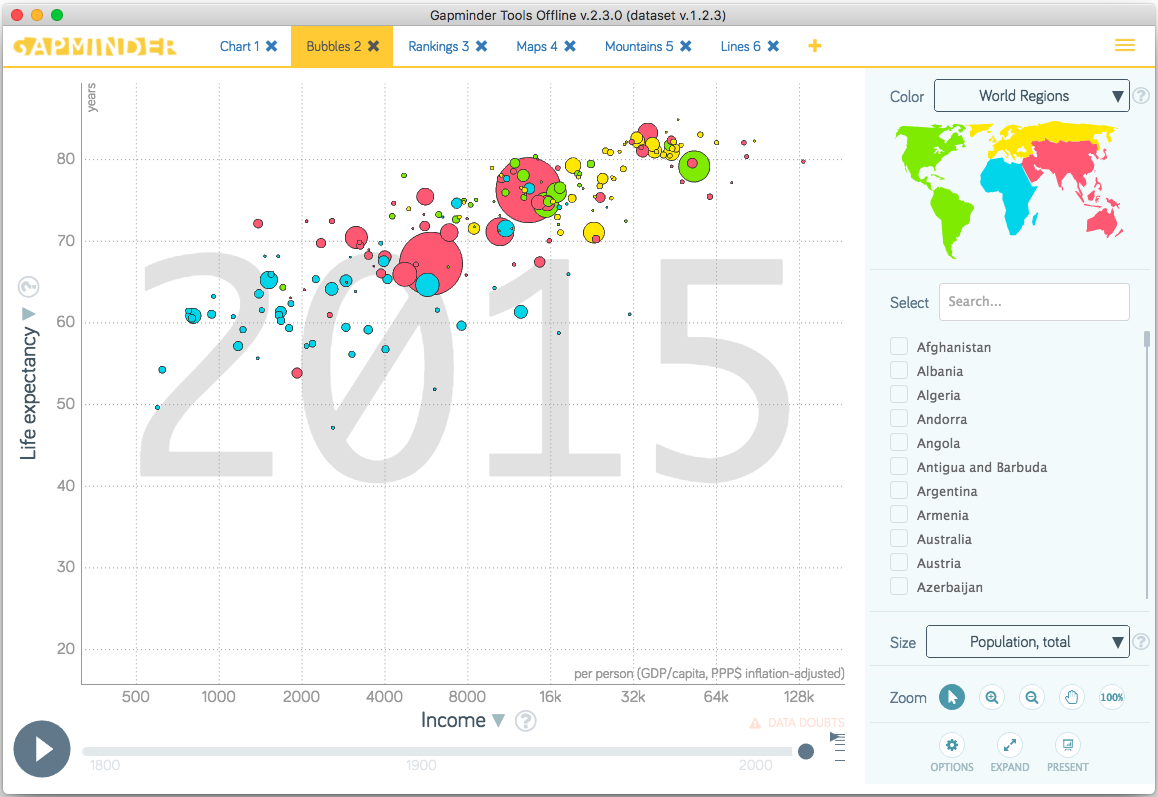
\includegraphics[width=0.95\columnwidth]{figures/bubbles}
	\caption{Chart of type ``bubbles'' in Gapminder.}
	\label{fig:bubbles}
\end{figure}

The visual variables being used are: position, size, color, text labels, animations and transparency.

\paragraph{Position}
The position is used to encode the value of $2$ indicators:
the position along the x-axis encodes the first indicator (in our case the income), the position along the y-axis the second one (in our case the life expectation).
Each point in the chart corresponds to a pair of income and life expectation.
By default, Gapminder limits the range of values showed on each axis between the smallest and the biggest value for the attribute displayed on that axis (plus some additional margin to make sure points do not overlap with the axises).
It is possible, if needed, to manually change the ranges using the ``Options'' menu at the bottom of the right side panel.

Each bubble in the chart represents a country.
Position is a very powerful visual variable: it is associative, selective, ordinal and quantitative.
The user will thus:
\begin{itemize}
    \item Distinguish relatively easily different points (i.e. different countries).
    \item Perceive each point independently of the other visual variables used. This allows to use other variables (eg. color or size) to encode additional dimensions of the data.
    \item Be able to easily order the points. This allows to easily tell which countries have lowest and highest values for one indicator and order the countries based on some indicator.
    \item Be able to easily compute ratios between the values of the indicators encoded by each point. This allows to compare the situation of pairs of different countries from the point of view of the $2$ indicator.
\end{itemize}

Please note that there are some limitations with this encoding.
For example, countries with the same income and life expectation will be shown in the same position:
it would be impossible for the user to distinguish them.
Also, bubbles with a big size tend to overlap with the others (since they take a lot of space on the screen).
Gapminder tries to reduce this problem in $2$ ways:
it shows smaller bubbles above bigger bubbles and it interactively shows the name of the countries in a label when the user moves the mouse on a bubble.

Overall, the encoding is good:
it uses a single visual variable (position) to represent $2$ dimensions of the dataset.
Although it is possible, it is unlikely that $2$ or more countries have exactly the same income and life expectation.
Gapminder takes some measures to reduce the problem of overlapping bubbles.
It also allows to encode, with some limitations, other attributes in size and color.

Additionally, the position visual variable is used in the colormap for the world's regions, as explained in the colors paragraph.

% TODO: we can force the tool to use categorical data for x-axis / y-axis !!! BAD

\paragraph{Size}
The size is used to encode the third indicator, in our case the population size.
In particular, the value is encoded as the area of the bubble.

Size is selective, ordinal and quantitative.
The user can thus:
\begin{itemize}
    \item Easily perceive countries with different populations as different from each other.
    \item Easily order countries by population size.
    \item Easily compute ratios between the size of the populations of different countries.
\end{itemize}

However, the tool does not visualize a legend for the sizes of the bubble.
This makes difficult to perform the inverse mapping from area of the bubble to size of the population by just looking at the bubble chart.
The value is visualized on the right side of the screen only if the user moves the mouse over a bubble.

The encoding of the population sizes is overall clear, but it can be improved.
On the one hand, the user is able to distinguish and compare the population of different countries.
On the other hand, it is quite complex to visualize the real values of the populations.

\paragraph{Color}
\label{paragraph:bubbles-color}
The color can be used to encode any of the available dimensions of the dataset.
In our case, the tool uses the color to encode the world region to which each country belongs.
Gapminder shows a colormap in the top right corner of the windows:
the colormap is visualized a small stylized planisphere where each continent if filled with the color that corresponds to its region.
The tool differentiate $4$ world regions: americas, africa, europe and russia, asia and oceania.

The colormap is categorical and uses different color hues for each different value.
The visualization uses the following $4$ colors: green, blue, yellow, red.
The choice of the color is good, since they are all distinct.
On the other hand, this choice does not take into account colorblind people that might have difficulties to distinguish green and red.
There is no way to change the colormap or force a different mapping.

Each bubble has a black border:
this makes it easier to identify a bubble and distinguish it from the other ones.
The visualization uses a white background, with a big gray text label in the center (to visualize the year, see the animation paragraph).
This is a good design choice, since it is a neutral color that does not interfere with the visualization and creates a high contrast with the colors used for the bubbles.

The encoding is clear: the $4$ choses colors are very different from each other, so it is very easy to distinguish point that corresponds to countries in different regions.
The inverse mapping from color to region of the world is also pretty straightforward, since there are only $4$ possible regions.

The color of a bubble together with the colormap allows to match each country with a specific location on the planisphere.
In other words, this allows the user to approximately locate the geographical position of each county.

\begin{figure}[h]
	\centering
	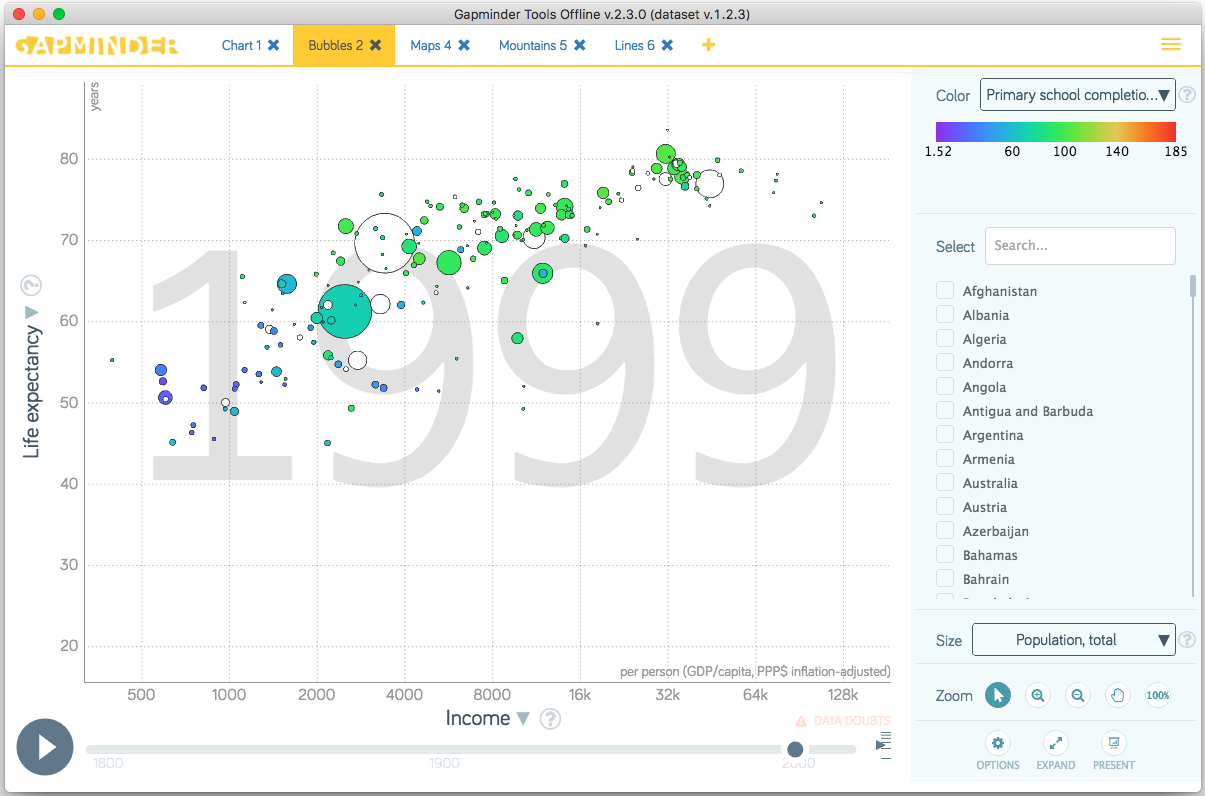
\includegraphics[width=0.95\columnwidth]{figures/bubbles-continuous-color}
	\caption{Use of color to encode a continuous data attribute in a chart of type ``bubbles'' in Gapminder.}
	\label{fig:bubbles-continuous-color}
\end{figure}

Gapminder allows to change the attribute encoded in color.
\cref{fig:bubbles-continuous-color} shows an example where color is used to encode the percentage of children that complete the primary school.
Gapminder automatically detects that the type of attribute is continuous and changes the color map to a continuous rainbow colormap, ranging from violet to represent the minimum value to red that to represent the maximum. It is possible to choose between the linear or a logarithmic scale using the dedicated menu; by default the tool uses a linear scale.

This encoding is not optimal:
rainbow color maps have been proven to be confusing (due to the non-obvious ordering of colors) and misleading (since it creates bands of colors with almost constant hues and sharp transitions in between) \cite{color-maps}.

In case the attribute mapped to color is missing, Gapminder shows a white bubble with a black border.
This is a good design choice, since white is a neutral color that does not interfere with the other colors.

\paragraph{Text Labels}
Text labels are used to show the name of the indicator visualized on the axises, the measure units and the value for the ticks.
The measure unit is shown above to the right for the x-axis.
Below the axis there are the values for the ticks (about $10$).
Below them in the center there is the name of the indicator.
All labels are gray.
The y-axis is similar.

Labels are used to visualize additional information about the bubbles.
When the user selects a particular bubble (either by moving the mouse over it, clicking it or selecting the checkbox of the corresponding country in the right panel), a text label is shown to the top right of the bubble.
The text label contains the name of the country, followed by the year.

Additionally, $2$ dashed lines parallel to the axis are displayed when the mouse pointer is over a bubble.
The lines start to from the bubble and intercept respectively the x and y-axis.
A new text label with the value for the indicators of the country that corresponds to the bubble is shown at the intersection with the axis.
This is a good design choice, since it allows the user to easily obtain additional information about interesting countries without polluting the visualization with the details about all the countries.

\paragraph{Animation}
Animation is used to show encode time.
Opposite to x-axis, y-axis, color and size, it is not possible to change the dimension of the dataset encoded with the animation.

The animation is started by pressing the ``play'' button in the bottom right corner of the windows.
When the animation is running, bubbles change position, size and color according to the new value of the corresponding indicators.
The slider on the bottom and the label with the year in the background change respectively position and value to reflect the time to which the indicators refers.
The ``play'' button changes icon to ``pause'': the user can stop the animation by pressing it again.
A small control to the right of the slider allows to change the speed of the animation.

\begin{figure}[h]
	\centering
	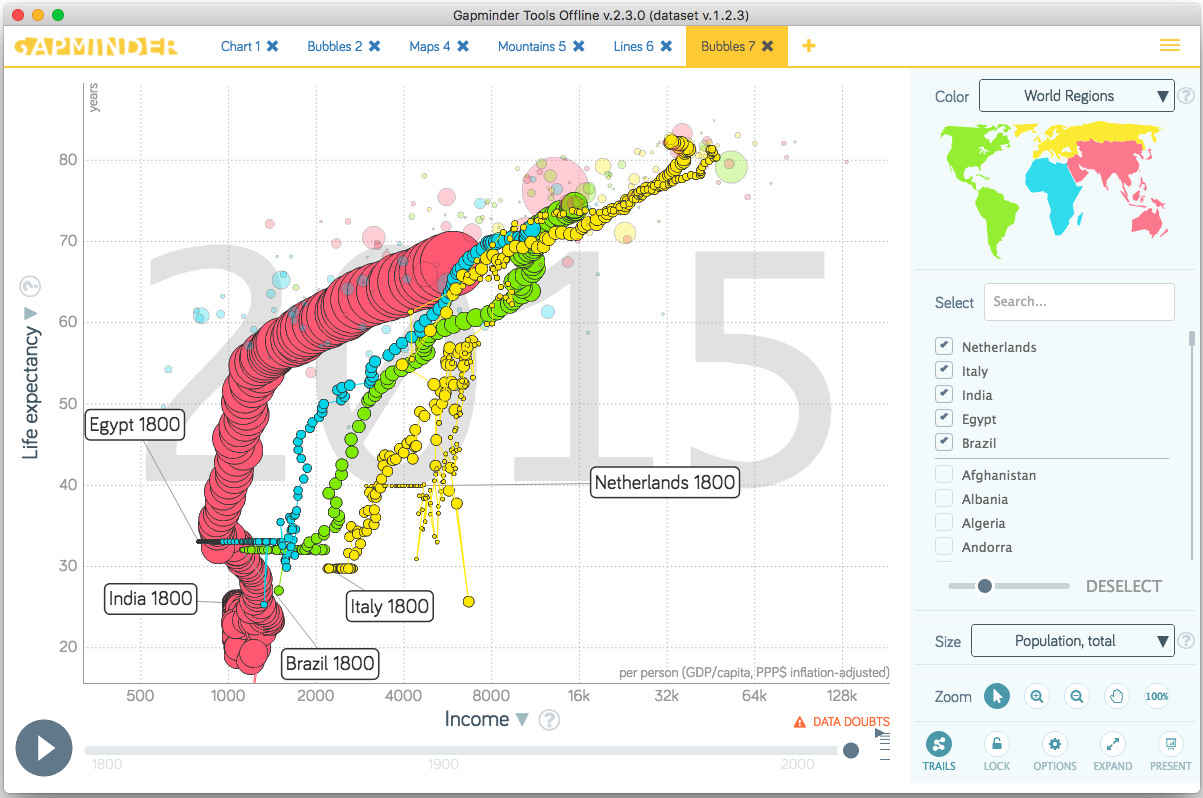
\includegraphics[width=0.95\columnwidth]{figures/bubbles-animation}
	\caption{Animation in a chart of type ``bubbles'' in Gapminder.}
	\label{fig:bubbles-animation}
\end{figure}

The user can also select one or more countries before running the animation.
In this case, Gapminder shows multiple bubbles for each selected countries, in particular one for each year the animation is played.
Successive bubbles are connected by a line of the same color of the bubble (if they do not partially overlap already).
The unselected countries are ``hidden'' by reducing their level of transparency (see the next paragraph).

This features allows the user to visualize better visualize trends.
One can first play the animation without selecting any particular country to can an idea about the general trend, and then select a group of countries of interest:
Gapminder will visualize the evolution over time for the selected countries (\cref{fig:bubbles-animation}).
This makes also easy to compare the evolution of the situation of some countries during time.

Animations are very powerful, but come with some drawbacks.
In the example shown in \cref{fig:bubbles-animation}, the problem of overlapping described in the position paragraph is heightened.
This is particularly true for bubbles with a big size (India in our example);
an expert user can reduce the problem by changing the scale size for the bubbles using the ``Options'' menu.
Nevertheless, animations are really effective to visualize changes and trends in the indicators over time.

\paragraph{Transparency}
Transparency does not encode any attribute of the dataset, but it is used to temporarily hide elements from the visualization.
When the user selects some bubbles, the unselected ones are hidden by reducing their level of transparency.
A slider is shown in the right panel and allows to change the transparency level.

This is a very good design choice, since it solves the problem of too many / overlapping bubbles and allows the user to focus on some particularly interesting country (or group of countries).
The same argument is valid during animations.


\subsubsection{Maps}
Gapminder's ``maps'' visualize the value of an indicator as a bubble centered in each country on a simplified world map (in the background).
\cref{fig:maps} shows a chart of type ``maps'' that visualizes the population size of the different countries.
The visual variables used are position, size, color, text labels, animation and transparency.
The encodings for size, text labels and transparency are the same as for the ``bubbles'', so we skip them here.

\begin{figure}[h]
	\centering
	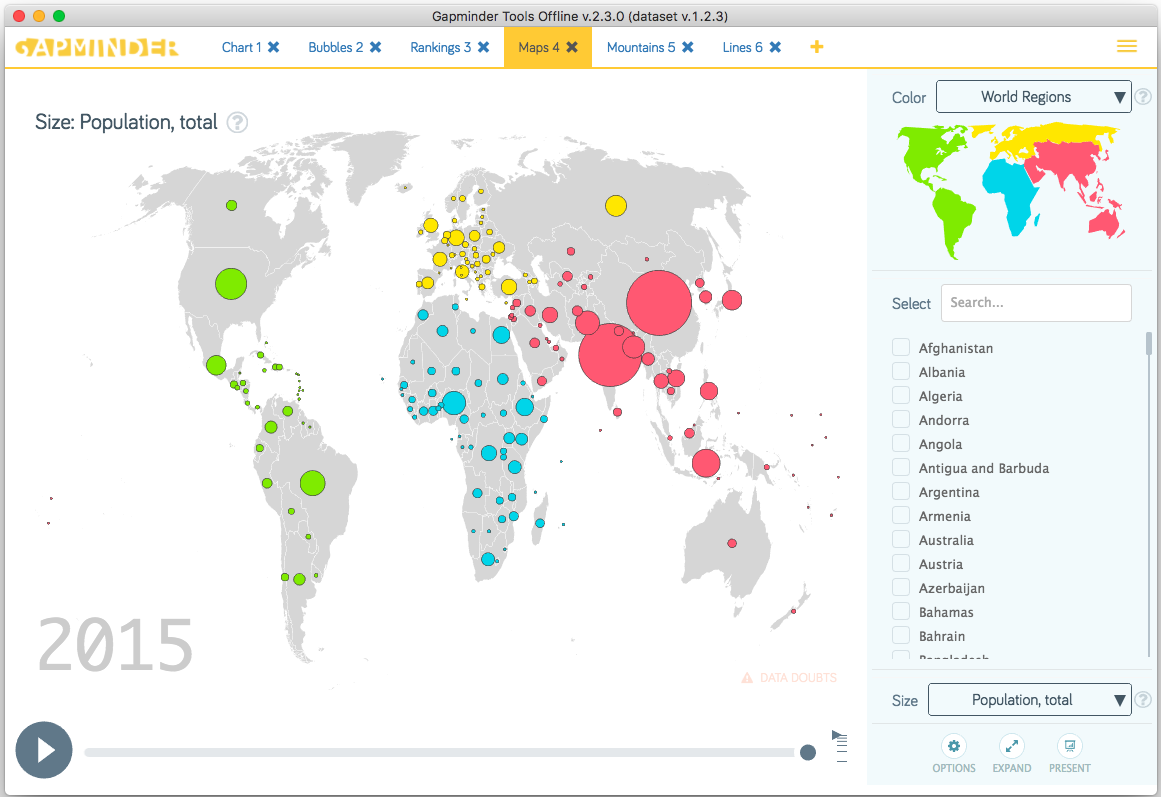
\includegraphics[width=0.95\columnwidth]{figures/maps}
	\caption{Chart of type ``maps'' that shows the population size of the different countries in Gapminder.}
	\label{fig:maps}
\end{figure}

\paragraph{Position}
The position is used to encode the geographical location of a country:
each bubble is centered in the center of the country to which it refers.
This allows to both easily compare the situation of countries which are located closed to each other.
The encoding is very clear, but it has the same problem of overlapping of bubbles presented in the \cref{subsubsec:bubbles}:
the problem particular present for europe and africa, since there are many countries in a relatively small area.

\paragraph{Color}
By default, color is used to encode the geographical region of the countries, like for the ``bubbles'' chart.
The encoding is clear, but it does not make much sense here, since the same information is encoded already in position.
This overloading wastes an important visualization variable that can be used to represent another dimension of the dataset.

Gapminder allows to change the dimension encoded in color using the corresponding menu.
The same discussion about color in \cref{subsubsec:bubbles} applies here as well.

\paragraph{Animation}
Animation is used to show encode time.
Like for the ``bubbles'' chart, the animation is controlled using the ``play'' / ``pause'' button and the slider in the bottom.
During the animation, the bubbles only changes size and color, but not the position, since it encode the country (which is the independent variable).
For the same reason, selected countries do not have any particular behaviour during the animation, as opposite to the ``bubbles'' chart.


\subsubsection{Mountains}
\begin{figure}[h]
	\centering
	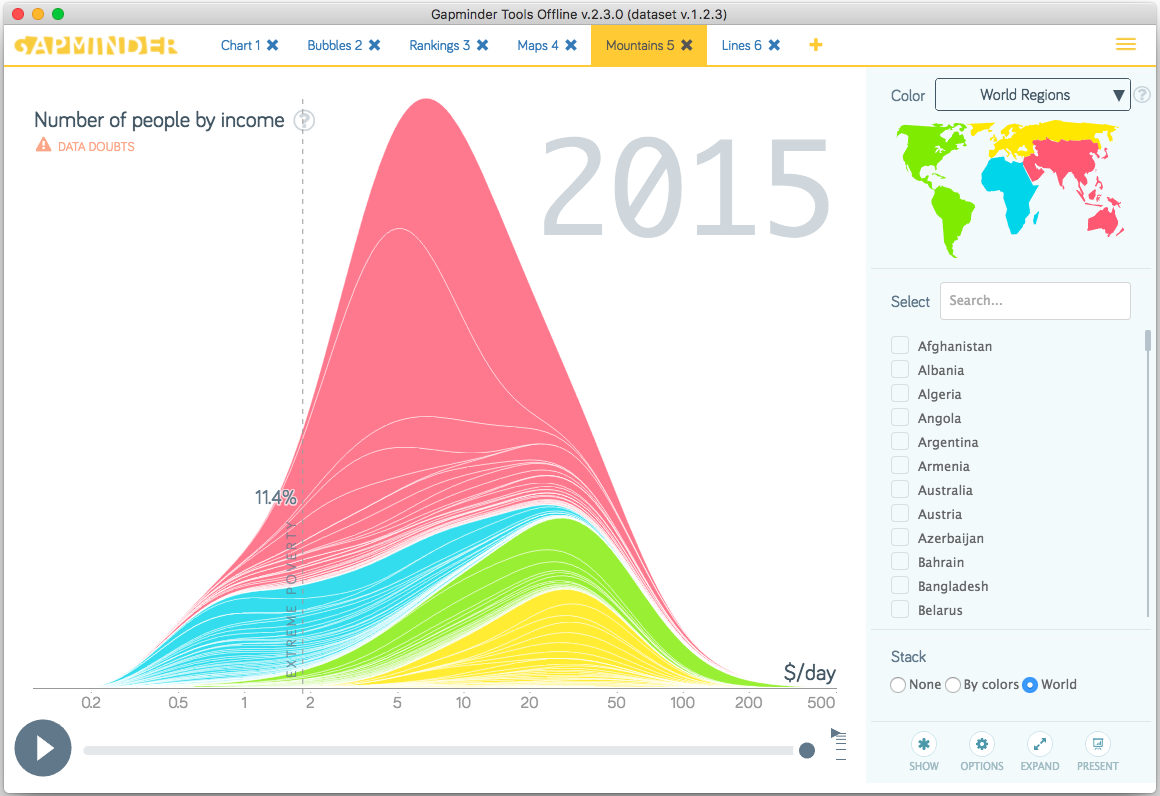
\includegraphics[width=0.95\columnwidth]{figures/mountains}
	\caption{Chart of type ``mountains'' with stacked areas in Gapminder.}
	\label{fig:mountains}
\end{figure}

Gapminder's ``mountains'' are area charts with animations.
This type of chart is used to show the distribution of number of people by income (measured as \$ / day).
Opposite to the other chart's types, Gapminder does not allow to change the indicator displayed.
% TODO: this means an extra data model!
Gapminder allows to choose not to stack the areas, stack them by color (this option is enables only if the color mapping is categorical) or stack them all.
\cref{fig:mountains} shows a screenshot of the ``mountains'' chart with stacked areas that shows the distribution of number of people by income.
The visual variables used are position, size, color, text labels, animations and transparency.

\begin{figure}[h]
	\centering
	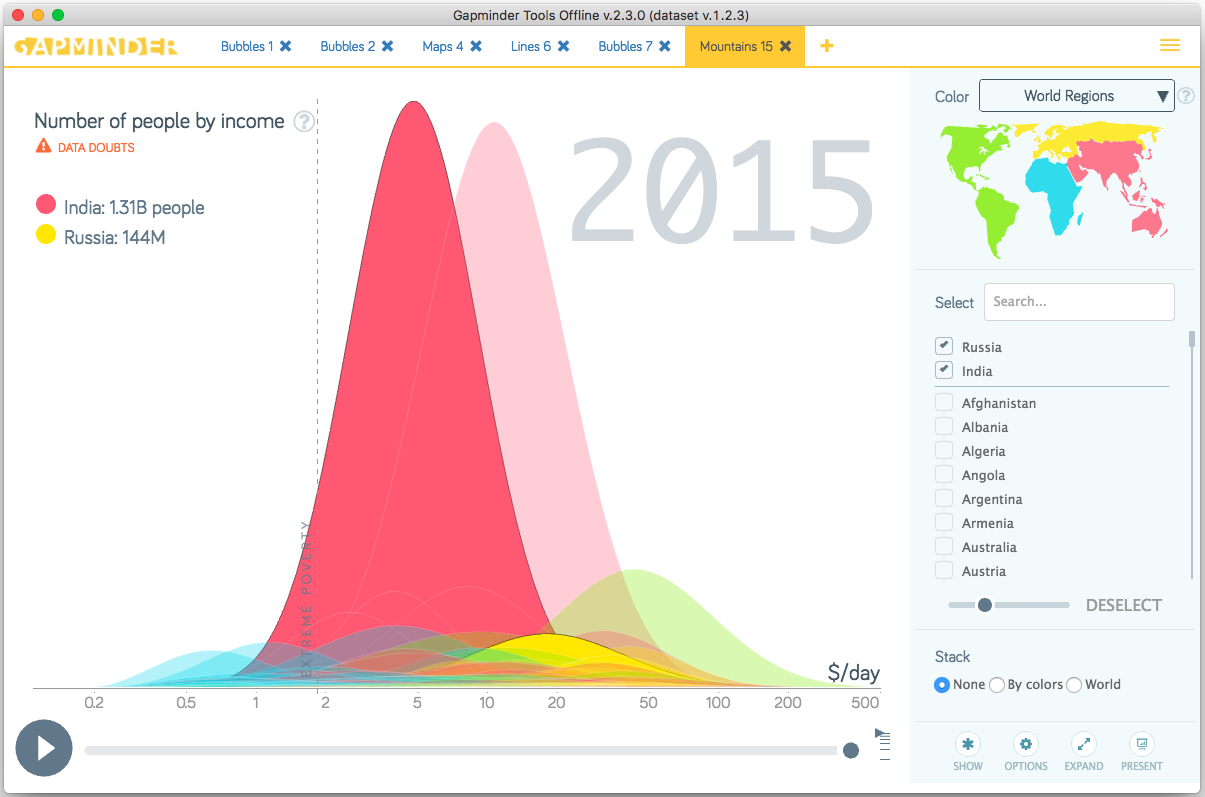
\includegraphics[width=0.95\columnwidth]{figures/mountains-non-stacked}
	\caption{Chart of type ``mountains'' with non-stacked areas in Gapminder.}
	\label{fig:mountains-non-stacked}
\end{figure}

\paragraph{Position}
Along the x-axis, position represents the daily income of the people on a logarithmic scale.
Along the y-axis. position assumes different meanings depending if areas are stacked or not.
If areas are not stack, the position along the y-axis indicates the number of people with some given income (determined by the position along the x-axis).
If areas are stacked, the meaning is more complicated:
it is still related to the number of people by income, but the value is measured starting from the point more in the bottom in the area for the fixed x-coordinate.
In other words, the meaning of each point in the stacked version depends on the shape of the area where it is contained.

Assuming basic knowledge of logarithms, the encoding along the x-axis is clear and easy to invert:
the user can simply use the ticks and labels along the x-axis to figure out the daily income value represented by a point.
However, Gapminder does not explicitly state that the scale is logarithmic, which may be confusing for the general public.

For the non-stacked version, the mapping along the y-axis is clear: the distance from the x-axis is proportional to the number of people with some income.
This allows the user to relatively easily compare the number of people with a certain income in different countries and compute approximate ratios.
For example, one could say that the number of people with an income between $5$ and $10$ \$/day in China and India in $2015$ is about the same.
However, it is difficult of impossible to read the absolute values, i.e. get how many people have a certain income in one country, since there is no explicit scale for the y-axis.

For the stacked version, the encoding along the less y-axis intuitive, but allows to easily compute aggregations:
the distance from the x-axis of each point represents the sum of people with the given income in all countries stacked together.
From \cref{fig:mountains} it is possible to say that most people in the world have an income between $5$ and $10$ \$/day in $2015$.

The non-stacked version has overlapping problems:
countries with similar income's distributions result in overlapping areas with a similar shape.
The problem is only partially solved by allowing the user to select only some countries (using the menu in the right panel).
\cref{fig:mountains-non-stacked} shows an example of non-stacked areas in Gapminder:
we have selected China and Nigeria to highlight them, but there are still clear overlapping problems, especially for Nigeria.

\paragraph{Size}
The size of an area encodes the size of the population of the corresponding country, both in the stacked and non-stacked versions.
The encoding allows to approximately compare the sizes of population of different countries.
However, this encoding is not clear for $2$ reasons:
\begin{itemize}
	\item The scale logarithmic along the x-axis deforms the areas.
	\item There is no legend for the sized of the areas.
\end{itemize}

\paragraph{Color}
The encoding of color is the same of the one for ``bubbles'' charts discussed in \cref{subsubsec:bubbles}.
This encoding has a problem in the non-stacked areas version:
when some countries are selected, the others are partially hidden by changing their level of transparency.
Overlapping areas with different colors and a non-zero level of transparency create new colors which does not belong to the color mapping.
This problem is evident with categorical color mapping:
in \cref{fig:mountains-non-stacked}, the overlapping of red area that represents China with the big green area on the right generates a big orange area.

\paragraph{Text Labels}
Labels are used for different scopes:
\begin{itemize}
	\item The title on the top-left part of the window gives a description of the visualization.
	\item The big text label with the year in the top-right part of the window display the year in which the population income is measured.
	\item The numbers below the x-axis indicate the daily income for points with the corresponding x-coordinate. This is fundamental for the inverse mapping from the position along the x-axis to the absolute value of daily income.
	\item A label above the x-axis indicates the measure unit used for the x-axis.
	\item When the user selects some countries, some text labels are displayed under the title (see \cref{fig:mountains-non-stacked}): they provide a color legend for the selected countries and indicate the population size.
	\item Finally, labels are display when the user moves the mouse on a particular area to indicate the name of the corresponding country.
\end{itemize}
All labels use neutral color (white, gray or black) not to attract the attention.
This is a good design choice, since it allows the user to focus on the visualization.

\paragraph{Animation}
Animation is used to show encode time.
Like for the ``bubbles'' chart, the animation is controlled using the ``play'' / ``pause'' button and the slider in the bottom.
During the animation, position, size, color and text labels are updated to reflect the data of the visualized year.

Animation allows the user to understand how the distribution of incomes in different countries has changed in time.
If the user is interested in particular countries, it can select and highlight them.

If no country is selected during the animation for the stacked version, countries in the same region are combined together.
This allows the user to understand the changes and trends for different regions in the world.
However, this encoding get really difficult to understand if the user changes the attribute encoded in color.
\cref{fig:mountains-animation} shows an example where color encodes the average income per person:
the user has no way to understand the meaning of different areas, since there are neither a legend nor labels to indicate it.

\begin{figure}[h]
	\centering
	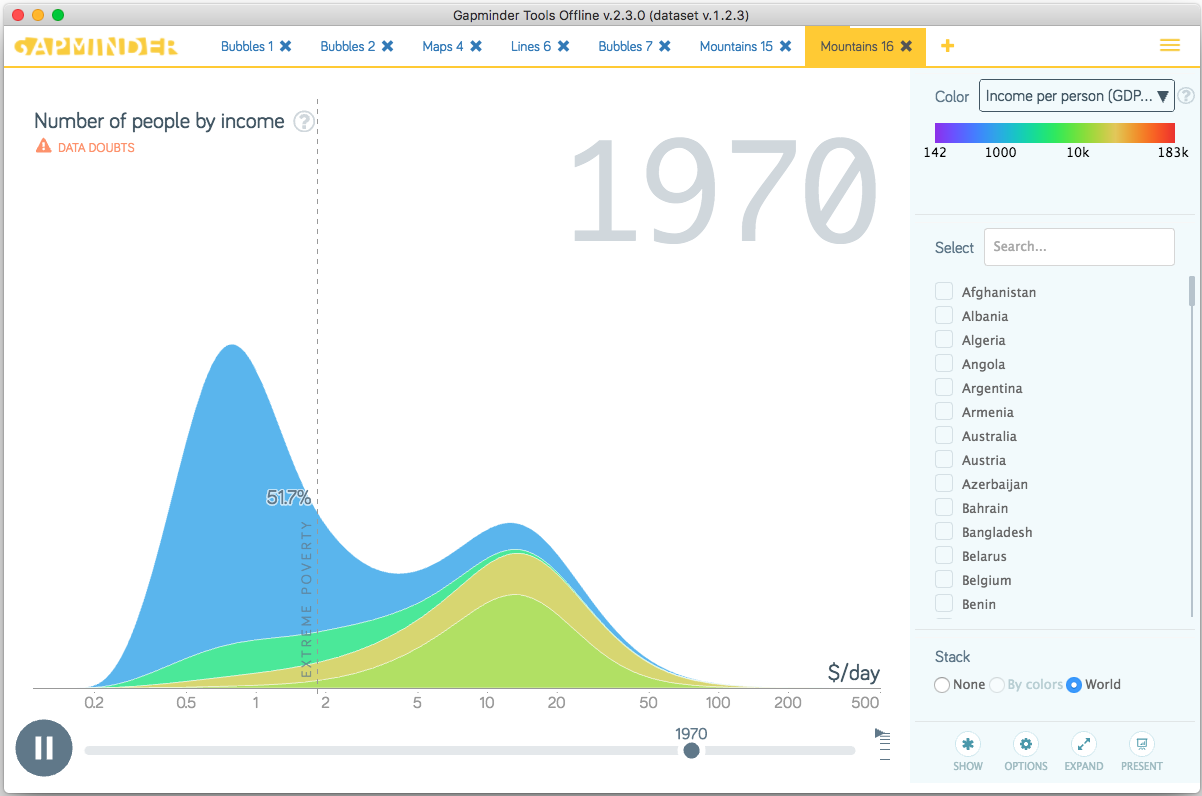
\includegraphics[width=0.95\columnwidth]{figures/mountains-animation}
	\caption{Chart of type ``mountains'' with stacked areas in Gapminder. The screenshot is taken during an animation.}
	\label{fig:mountains-animation}
\end{figure}

\paragraph{Transparency}
The encoding of color is the same as the ``bubbles'' charts discussed in \cref{subsubsec:bubbles}.
We have discussed the problems of combining transparency and color in the color paragraph.


\subsubsection{Rankings}
Gapminder's ``rankings'' are bar charts with animations.
Each bar corresponds to a country.
The bar charts is oriented horizontally.
The visual variables used are position, size, color, text labels, animations and transparency.
The encodings for color and transparency are the same as for the ``bubbles'', so we skip them here.

\begin{figure}[h]
	\centering
	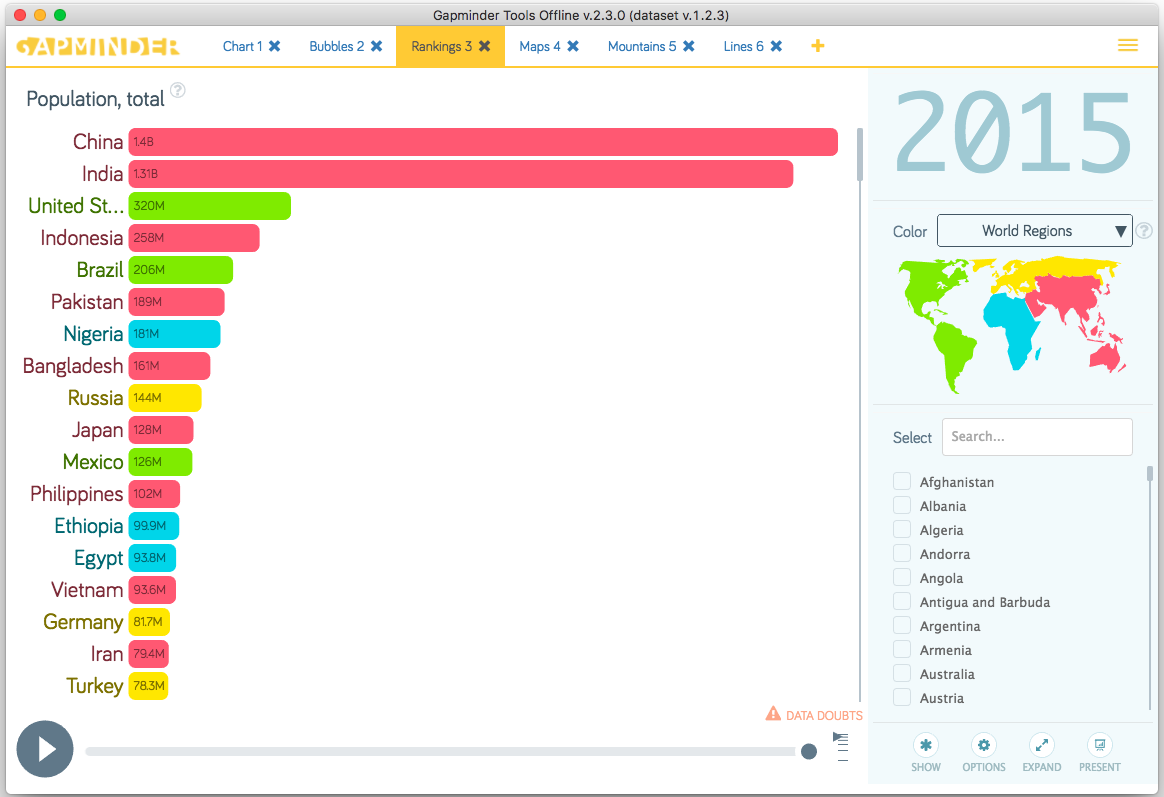
\includegraphics[width=0.95\columnwidth]{figures/rankings}
	\caption{Chart of type ``rankings'' in Gapminder.}
	\label{fig:rankings}
\end{figure}

\paragraph{Position}
Position is used to encode the ranking of countries by the value of the indicator encoded in size.
Countries are ordered for decreasing values:
countries with higher values are located at the top, the ones with lower values at the bottom.
It is not possible to change the ordering, i.e. put the countries with lower values at the top.
Countries without data for the indicator are put to the bottom.

The encoding allows the user to easily find the top countries and the ones with the smaller values for the displayed indicator, although this usually requires to scroll down with the mouse (since a normal size screen is not long enough to display all bars).
It is also allows to compare pairs of countries in the ranking for the indicator.
In this sense, the encoding is good.

\paragraph{Size}
Size is used to encode an indicator, such as the size of the population.
The length of each bar is linearly proportional to the value of the indicator.
It is possible to change the scale to logarithmic by clicking on the title of the chart, above the first bar.

The user is able to:
\begin{itemize}
	\item Order countries by the value of the indicator.
	\item Compute ratios between the value of the indicator for different countries. In the example of \cref{fig:rankings}, the user can for example estimate the population of China to $3$ to $4$ times bigger than the one of the United States.
\end{itemize}

The encoding is good for ordering and computing rates.
However, it is not easy to extract the absolute value of a bar, since there is no length legend.
This information is only encoded in text labels inside each bar, but they are not always easy to read.

\paragraph{Text Labels}
Text labels does not encode directly any dimension, but are fundamental for different aims:
\begin{itemize}
	\item The title of the chart indicates which indicator is encoded in the length of the bar.
	\item The labels before each bar indicates which country the bar refers to.
	\item The labels inside each bar report the value of the indicator measured in the corresponding country.
	\item A big text label in the top part of the right panel indicates in which year are measured the displayed data.
\end{itemize}

The labels with the country names and those inside the bars have the same color hue of bar to which they refer (with a slightly higher saturation).
On the one hand, this makes easier to associate them with the correct bar.
On the other hand, it is particularly difficult to read the labels inside red and blue bars due to the low contrast.

\paragraph{Animation}
Animation is used to show encode time.
During the animation, position, size, label and labels of the bars are updated to reflect the displayed year.
The user can select one or more countries to highlight them:
in this case, Gapminder will also automatically scroll the view if the selected bars exits the current one.

The animation allows to track the evolution of the selected countries over time.
However, it does not allow to have a visualize the global trend, since there are too many variations (also, not all bars fit in the size of a the monitor).
It is also difficult to compare $2$ or more countries, since small changes in the measured value can cause significant changes in the ranking and / or a swap in their relative order: tracking all these variations over successive visualizations is hard.
For this kind of task, the chart of type ``bubbles'' is to be preferred.


\subsubsection{Lines}
Gapminder's ``lines'' are line charts with animations.
They show the variation of one indicator over time:
the x-axis represents time (in years), while the y-axis a given indicator.
\cref{fig:lines} shows a Gapminder ``lines'' chart visualizing the average income of different countries over time.
By default, only some countries are shown;
the user can change the selected countries using the menu in the right panel.

The visual variables used are position, color, text labels and animation.
The encoding for the color is the same as for the ``bubbles'', so we omit it here.
Transparency is not used in this type of chart:
only the selected countries are visualized, the others are not drawn.

\begin{figure}[h]
	\centering
	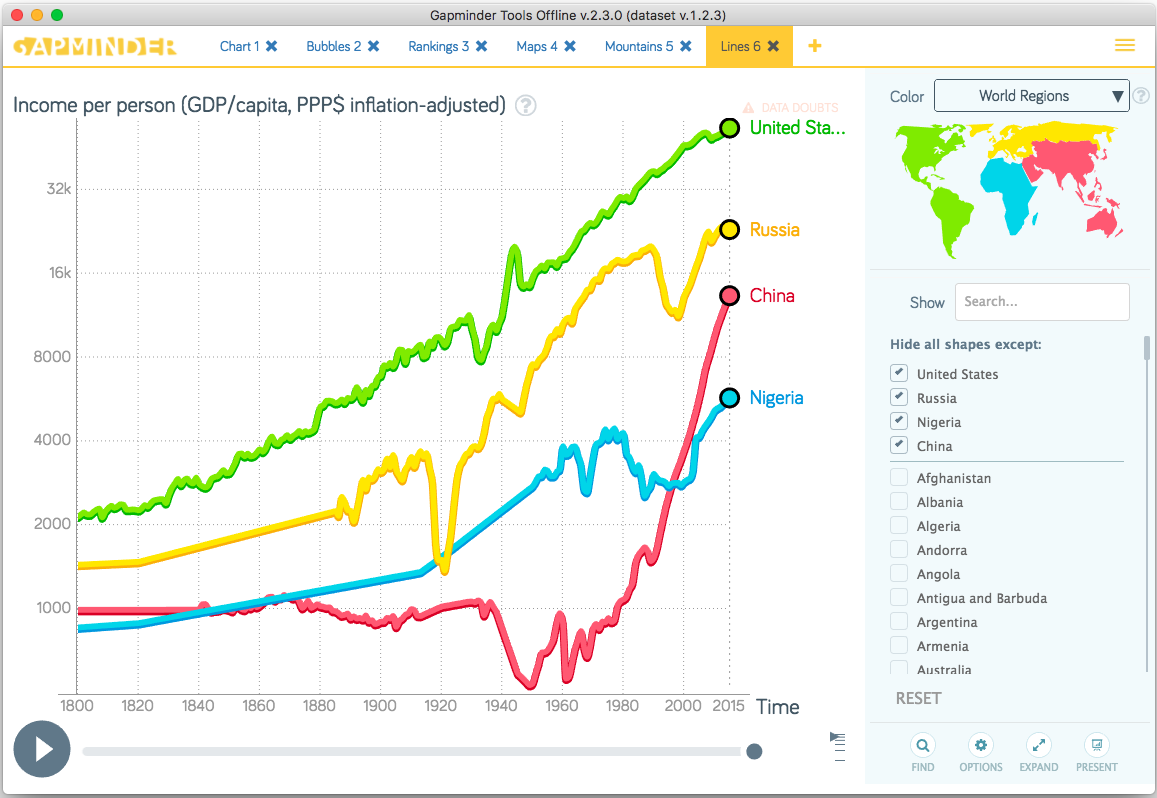
\includegraphics[width=0.95\columnwidth]{figures/lines}
	\caption{Chart of type ``lines'' in Gapminder.}
	\label{fig:lines}
\end{figure}

\paragraph{Position}
Position is used to encode the pair time (along the x-axis) and the selected indicator, for example income per person in \cref{fig:lines}.
The encoding is very clear and effective:
each point in the chart has a one-to-one mapping with a the pair time and income.
The encoding is easy to reverse thanks to the dashed gray lines in the background, the ticks and the labels on the axises.

\paragraph{Text Labels}
Text labels are used for:
\begin{itemize}
	\item Describe the dimensions and measure units represented by the axises.
	\item Provided a legend for the plotted line (each line has a label with the name of the country closed to the end of the line).
\end{itemize}
The use of labels is fundamental for the inverse mapping of position and color.

\paragraph{Animation}
Animation encodes times.
In this type of chart, time is already encoded in the x-axis.
The animation does not show any new information, but simply make the drawing of the line interactive:
when the user starts the animation, lines are removed;
at each step of the animation, lines are drawn from the first year to the current year in the animation.
\cref{fig:lines-animation} shows an example of line chart when the animation reaches year $1935$.

The animation does not encode any additional information, so it is not really useful to display the data.
On the other hand, the animation does not have negative effects on the visualization, since the user can simply not use it.

\begin{figure}[h]
	\centering
	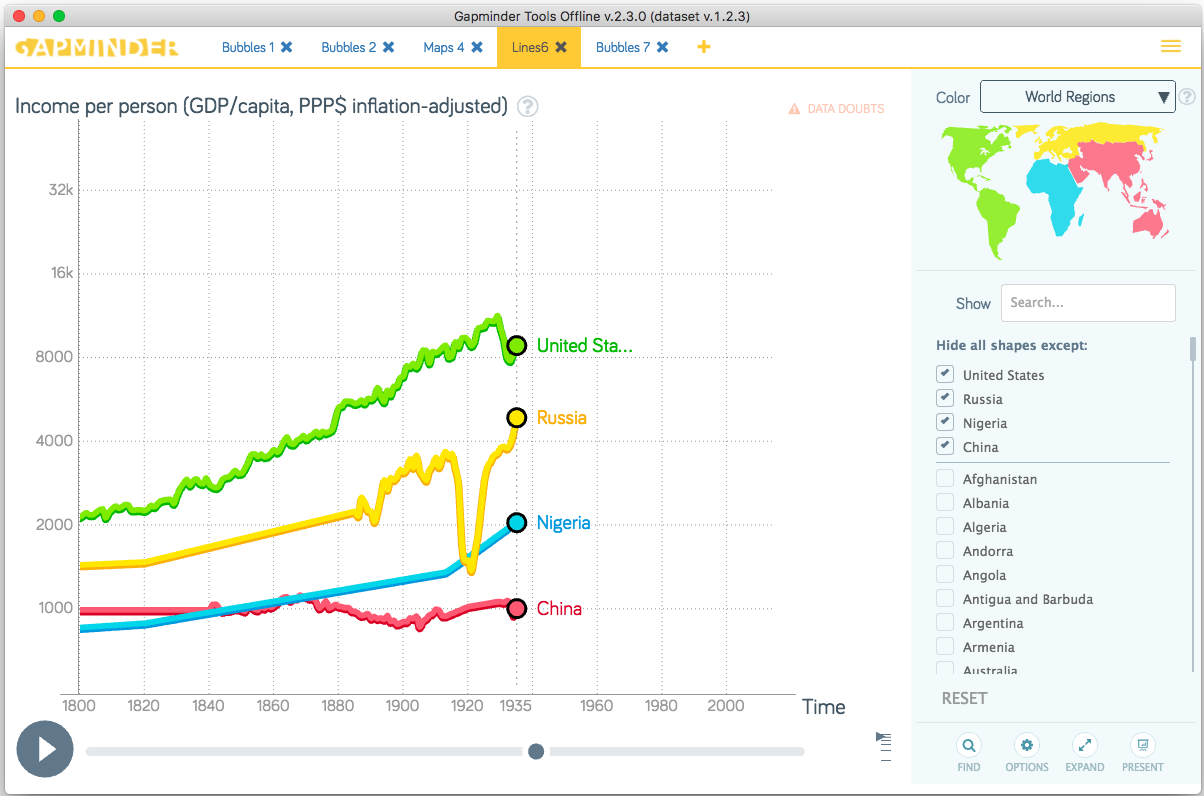
\includegraphics[width=0.95\columnwidth]{figures/lines-animation}
	\caption{Chart of type ``lines'' in Gapminder. The screenshot is taken during an animation.}
	\label{fig:lines-animation}
\end{figure}


\subsection{Improvements}
TODO...
Bullet list of points to discuss:
\begin{itemize}
    \item add a legend for the size of the bubbles
    \item add information about the 3 indicators in the tooltip of the bubble (proximity gestalt law)

    \item colormap... not easy to read for colorblind people... possibility to choose a different colormap for colorblind people, since there are only 4 colors
\end{itemize}
